\section{Results}
\label{sec:results}

All numbers below are generated from the run outputs by the released scripts; $\pm$ is the standard
deviation over runs. Differences are given as mean over matched fold--seed runs, with the number of
runs in which the first model wins and 95\% intervals as described in \cref{sec:experiments}.

\begin{table*}[t]
\centering
\caption{Main results (\%). Clean = in-domain grouped 5-fold accuracy; Rot.\ min = worst accuracy over
12 rotations; MedLeaf-C = mean over 10 corruptions $\times$ 3 severities; Shape bias from the
cue-conflict set; Field = 20-way accuracy on DIMPSAR field photographs (auto-masked or raw).
ConvNeXt-T: 5 folds $\times$ 5 seeds (MedLeaf-C: seeds 0, 3, 4, all seeds for mask pooling; Rot.\ min
and shape bias: seed 0); EfficientNet-B0: 5 folds
$\times$ 3 seeds; ViT-S and BioCLIP~2: 5 folds, one seed. Mask pooling was run on ConvNeXt-T only.}
\label{tab:main}
\small
\resizebox{\textwidth}{!}{\begin{tabular}{llcccccc}
\toprule
Backbone & Model & Clean & Rot.\ min & MedLeaf-C & Shape bias & Field (mask) & Field (raw) \\
\midrule
ConvNeXt-T & Plain & 99.9\,$\pm$\,0.1 & 99.9\,$\pm$\,0.2 & 81.1\,$\pm$\,1.1 & 6.5\,$\pm$\,1.5 & 35.1\,$\pm$\,1.3 & 33.5\,$\pm$\,1.2 \\
 & Global fusion & 100.0\,$\pm$\,0.1 & 99.7\,$\pm$\,0.3 & 81.0\,$\pm$\,0.8 & 7.0\,$\pm$\,1.9 & 34.9\,$\pm$\,1.7 & 33.7\,$\pm$\,1.3 \\
 & Strip pooling & 100.0\,$\pm$\,0.0 & 99.9\,$\pm$\,0.1 & 87.6\,$\pm$\,0.8 & 9.1\,$\pm$\,1.5 & 42.9\,$\pm$\,1.6 & 47.8\,$\pm$\,2.0 \\
 & Slab-only & 100.0\,$\pm$\,0.1 & 100.0\,$\pm$\,0.0 & 89.4\,$\pm$\,0.9 & 7.4\,$\pm$\,1.9 & 42.2\,$\pm$\,1.1 & 45.7\,$\pm$\,2.0 \\
 & SVA (ours) & 100.0\,$\pm$\,0.1 & 99.9\,$\pm$\,0.1 & 88.6\,$\pm$\,0.5 & 9.0\,$\pm$\,2.3 & 43.1\,$\pm$\,2.8 & 49.3\,$\pm$\,2.8 \\
\midrule
ViT-S/16 & Plain & 99.9\,$\pm$\,0.1 & 99.9\,$\pm$\,0.1 & 96.4\,$\pm$\,0.3 & 9.7\,$\pm$\,1.0 & 51.6\,$\pm$\,0.4 & 60.4\,$\pm$\,0.9 \\
 & Global fusion & 100.0\,$\pm$\,0.0 & 99.9\,$\pm$\,0.1 & 96.2\,$\pm$\,0.6 & 9.1\,$\pm$\,1.3 & 50.1\,$\pm$\,0.7 & 58.6\,$\pm$\,1.8 \\
 & Strip pooling & 99.9\,$\pm$\,0.1 & 99.9\,$\pm$\,0.1 & 96.2\,$\pm$\,0.5 & 10.3\,$\pm$\,1.3 & 51.2\,$\pm$\,1.1 & 62.7\,$\pm$\,1.0 \\
 & Slab-only & 100.0\,$\pm$\,0.0 & 99.8\,$\pm$\,0.1 & 96.6\,$\pm$\,0.5 & 11.0\,$\pm$\,1.4 & 52.0\,$\pm$\,0.8 & 64.8\,$\pm$\,2.1 \\
 & SVA (ours) & 99.9\,$\pm$\,0.1 & 99.9\,$\pm$\,0.1 & 96.6\,$\pm$\,0.3 & 9.3\,$\pm$\,1.8 & 51.9\,$\pm$\,1.0 & 60.7\,$\pm$\,1.4 \\
\midrule
BioCLIP 2 & Plain & 99.9\,$\pm$\,0.1 & 99.0\,$\pm$\,0.4 & 93.8\,$\pm$\,0.5 & 14.0\,$\pm$\,1.3 & 58.9\,$\pm$\,0.5 & 81.4\,$\pm$\,0.7 \\
 & Global fusion & 99.9\,$\pm$\,0.1 & 99.0\,$\pm$\,0.4 & 93.8\,$\pm$\,0.6 & 14.3\,$\pm$\,2.3 & 59.7\,$\pm$\,1.1 & 81.3\,$\pm$\,0.2 \\
 & Strip pooling & 99.9\,$\pm$\,0.1 & 99.2\,$\pm$\,0.5 & 93.8\,$\pm$\,0.2 & 14.2\,$\pm$\,1.7 & 58.9\,$\pm$\,0.7 & 81.5\,$\pm$\,0.5 \\
 & Slab-only & 100.0\,$\pm$\,0.0 & 98.8\,$\pm$\,0.5 & 93.9\,$\pm$\,0.6 & 13.9\,$\pm$\,1.2 & 60.7\,$\pm$\,0.7 & 81.8\,$\pm$\,1.4 \\
 & SVA (ours) & 100.0\,$\pm$\,0.0 & 98.5\,$\pm$\,0.5 & 93.5\,$\pm$\,0.5 & 13.7\,$\pm$\,2.0 & 59.8\,$\pm$\,1.1 & 81.7\,$\pm$\,0.8 \\
\bottomrule
\end{tabular}}
\end{table*}

\subsection{In-domain accuracy is saturated}
On the de-duplicated, grouped protocol every model on every backbone reaches 99.9--100\% clean
accuracy and $\ge98.5\%$ accuracy under any rotation (\cref{tab:main}). The studio benchmark therefore
cannot separate architectures, and none of the added modules costs clean accuracy. All further
results concern robustness and, primarily, transfer to field photographs.

\subsection{Decomposing the studio-to-field gain}
\label{sec:decomp}
\Cref{fig:crossdomain} and \cref{tab:contrasts} show the main result. A plain ConvNeXt-T trained on
studio images reaches 33.6\% on raw field photographs. The localised models reach 45.7--47.4\%, a gain
of 12--14 points. The ladder of matched models splits this gain into two parts of similar size.

\emph{Leaf location.} Pooling the same patch features over the leaf mask raises raw field accuracy to
41.1\% ($+7.5$ points, 25/25 runs, Holm $p<10^{-4}$), and masked-photo accuracy by $+5.7$. The plain
model averages features over the whole photograph, and on field photographs the background (tiles,
soil, cloth) is a large part of it; a model that knows where the leaf is can ignore it.

\emph{Localisation.} Pooling locally within the leaf adds a further 4.6--6.2 points on raw photographs:
strip pooling $+5.7$ (25/25, Holm $p=0.002$), slab-only attention $+4.6$ (24/25, Holm $p=0.008$) and
\SVA{} $+6.2$ (23/25; Holm $p=0.18$ because its run-to-run variance is the largest). The two-way
bootstrap over runs and field species excludes zero for all three. On masked photographs, where the
background is already removed, localisation adds only 1.2--1.6 points (not significant).

\emph{Measured geometry.} Adding the measured valuations to localised tokens does not help detectably.
\SVA{} is tied with strip pooling ($+0.5$, 12/25) and with its own slab-only variant ($+1.7$, 16/25),
with intervals of roughly $\pm4$ points around these values. Fusing the same valuations globally,
without localisation, gives no gain at all over plain ($-0.1$, 13/25). Object-centred sweep slabs
and image-axis strips perform the same.

\begin{figure}[t]
\centering
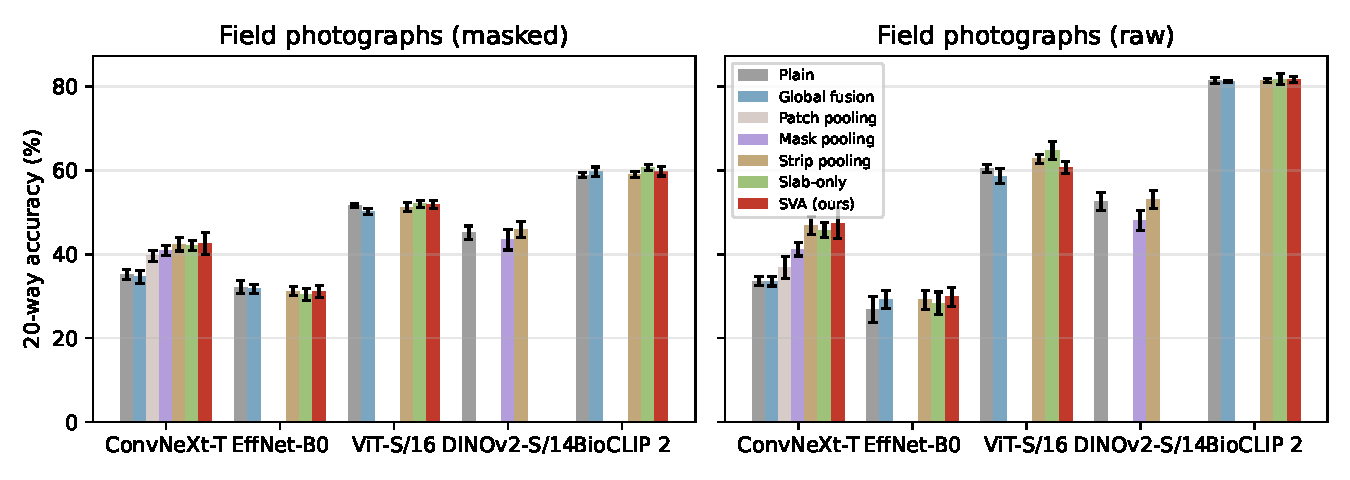
\includegraphics[width=\linewidth]{figures/fig_crossdomain.pdf}
\caption{Studio-to-field transfer: 20-way accuracy on DIMPSAR photographs with the background
whitened by our masker (left) or kept (right). Error bars: std over runs. Mask pooling was run on
ConvNeXt-T only.}
\label{fig:crossdomain}
\end{figure}

\begin{table}[t]
\centering
\caption{Pre-specified contrasts on field photographs (ConvNeXt-T, 25 matched runs). $\Delta$ in
accuracy points with runs won; 95\% intervals from the corrected resampled $t$-test over runs and from
a bootstrap over runs and field species; $p$ Holm-corrected over all 14 contrasts.}
\label{tab:contrasts}
\small
\resizebox{\linewidth}{!}{\begin{tabular}{llcccc}
\toprule
Photos & Contrast & $\Delta$ (points) & 95\% CI, runs & 95\% CI, runs+species & Holm $p$ \\
\midrule
raw & mask pooling $-$ plain & +7.5 (25/25) & [+5.3, +9.8] & [+3.0, +12.2] & $<10^{-4}$ \\
 & strip $-$ mask pooling & +5.7 (25/25) & [+3.0, +8.4] & [+2.3, +9.2] & 0.002 \\
 & slab-only $-$ mask pooling & +4.6 (24/25) & [+2.1, +7.0] & [+0.7, +8.9] & 0.008 \\
 & SVA $-$ mask pooling & +6.2 (23/25) & [+1.2, +11.3] & [+2.4, +10.2] & 0.18 \\
 & SVA $-$ slab-only & +1.7 (16/25) & [-3.5, +6.8] & [-2.8, +6.5] & 1.00 \\
 & SVA $-$ strip & +0.5 (12/25) & [-3.6, +4.7] & [-3.0, +4.5] & 1.00 \\
 & global fusion $-$ plain & -0.1 (13/25) & [-1.5, +1.3] & [-2.3, +2.4] & 1.00 \\
\midrule
masked & mask pooling $-$ plain & +5.7 (25/25) & [+3.6, +7.8] & [+2.3, +9.3] & 0.000 \\
 & strip $-$ mask pooling & +1.5 (21/25) & [-0.7, +3.7] & [-1.4, +4.3] & 1.00 \\
 & slab-only $-$ mask pooling & +1.2 (20/25) & [-0.7, +3.2] & [-2.4, +5.0] & 1.00 \\
 & SVA $-$ mask pooling & +1.6 (17/25) & [-1.7, +4.9] & [-1.7, +4.9] & 1.00 \\
 & SVA $-$ slab-only & +0.4 (15/25) & [-3.2, +3.9] & [-3.4, +4.4] & 1.00 \\
 & SVA $-$ strip & +0.1 (15/25) & [-3.4, +3.5] & [-2.9, +3.4] & 1.00 \\
 & global fusion $-$ plain & -0.6 (8/25) & [-2.4, +1.2] & [-3.4, +2.3] & 1.00 \\
\bottomrule
\end{tabular}}
\end{table}

\subsection{The gains are not an artefact of augmentation}
\label{sec:norot}
\label{sec:strongaug}
\emph{Without rotation augmentation} (5 folds $\times$ 5 seeds), the localised models remain far more
rotation-robust than plain (worst-case accuracy 97.5--98.4\% vs.\ 93.2\%; \cref{fig:rotation}) and
keep their field gain: plain 32.1\%, slab-only 43.2\%, strip 43.9\%, \SVA{} 45.5\% on raw photographs
(\SVA{} vs.\ plain $+13.5$ [$+9.7$, $+17.3$], 25/25). \SVA{} is again not distinguishable from strip
pooling ($+1.6$, 16/25) or slab-only attention ($+2.4$, 20/25). With a single seed these leads had
looked much larger ($+5.8$ and $+5.2$), which illustrates why we rely on many seeds.

\emph{With strong augmentation} (background compositing, blur, noise; \cref{tab:strongaug}), every
model improves: plain rises from 33.6\% to 42.0\% on raw photographs, about as much as mask pooling
gives without it, which is consistent with both teaching the model to discount the background.
Localisation still adds on top: strip pooling reaches 53.4\% and \SVA{} 55.2\%, the best field
accuracy of any ImageNet model here (\SVA{} vs.\ plain $+13.2$ [$+9.9$, $+16.5$], 15/15; vs.\ strip
$+1.9$, 13/15, n.s.). The architectural and data-side remedies are therefore complementary.

\begin{figure}[t]
\centering
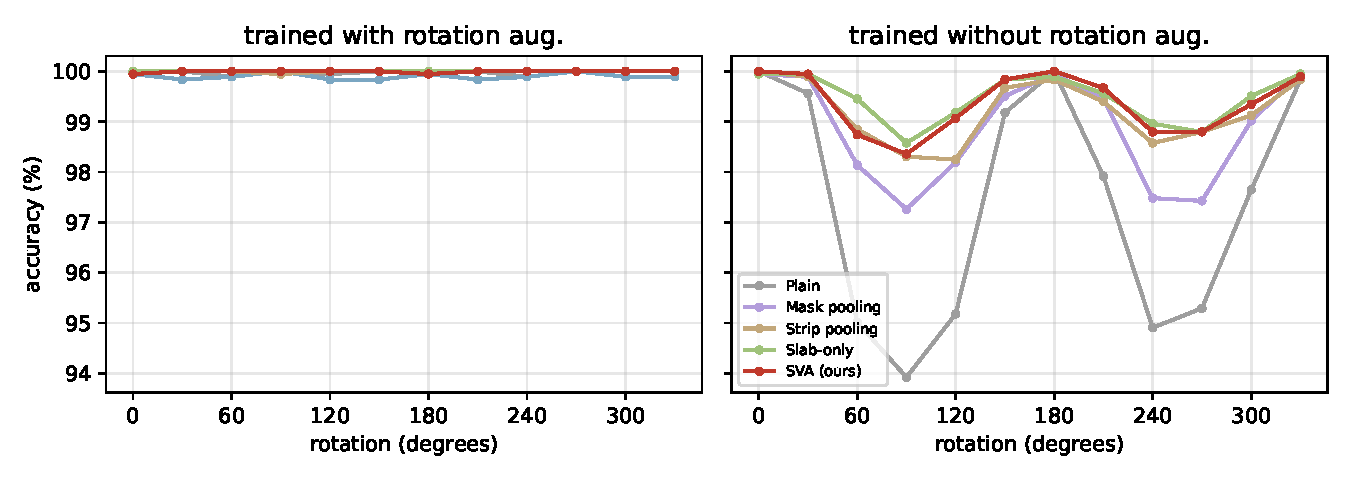
\includegraphics[width=\linewidth]{figures/fig_rotation.pdf}
\caption{Accuracy versus test-time rotation (ConvNeXt-T, seed 0, mean over 5 folds), trained with
(left) and without (right) rotation augmentation.}
\label{fig:rotation}
\end{figure}

\begin{table}[t]
\centering
\caption{Standard vs.\ strong (background compositing + blur + noise) augmentation, ConvNeXt-T,
5 folds $\times$ 3 seeds, \%.}
\label{tab:strongaug}
\small
\begin{tabular}{llccc}
\toprule
Augmentation & Model & MedLeaf-C & Field (mask) & Field (raw) \\
\midrule
standard & Plain & 81.1\,$\pm$\,1.1 & 35.1\,$\pm$\,1.3 & 33.5\,$\pm$\,1.2 \\
 & Strip pooling & 87.6\,$\pm$\,0.8 & 42.9\,$\pm$\,1.6 & 47.8\,$\pm$\,2.0 \\
 & SVA (ours) & 88.6\,$\pm$\,0.5 & 43.1\,$\pm$\,2.8 & 49.3\,$\pm$\,2.8 \\
\midrule
strong & Plain & 96.5\,$\pm$\,0.3 & 43.1\,$\pm$\,1.3 & 42.0\,$\pm$\,1.7 \\
 & Strip pooling & 97.9\,$\pm$\,0.1 & 49.3\,$\pm$\,1.3 & 53.4\,$\pm$\,1.7 \\
 & SVA (ours) & 97.8\,$\pm$\,0.3 & 49.4\,$\pm$\,1.7 & 55.2\,$\pm$\,2.0 \\
\bottomrule
\end{tabular}
\end{table}

\subsection{The gains depend on the backbone}
On EfficientNet-B0 (3 seeds) all four structural models gain only 1.5--3 points on raw photographs
(plain 26.8\%, \SVA{} 29.8\%, $+3.0$ [$-2.6$, $+8.6$], 11/15) and nothing on masked ones. On ViT-S,
localised pooling may still help (strip 62.7\%, slab-only 64.8\% vs.\ plain 60.4\%, one seed), but
\SVA{} does not (60.7\%). BioCLIP~2 reaches 81.4\% on raw photographs without any module, about
30 points above the best ImageNet ConvNeXt-T model, and all variants lie within 0.5 points of each
other. A biology foundation model thus closes most of the studio-to-field gap on its own. For both
ViTs, masked photographs are 8--22 points \emph{harder} than raw ones, whereas for the CNNs the two
differ by at most about five points; the whitened background and the masker's errors apparently remove context these models
use, so we treat raw photographs as the primary field test.

\subsection{Corruptions and cue conflict}
On MedLeaf-C (\cref{fig:corruptions}), the ladder repeats on ConvNeXt-T: mask pooling improves on plain
by $+2.7$ points (84.8\% vs.\ 82.1\%, 15/15), and localised pooling adds a further 2.2--4.0 (strip
87.5\%, \SVA{} 87.0\%, slab-only 88.8\%). The gains come from noise, blur, JPEG and low-resolution
corruptions, i.e.\ from degraded texture; colour, occlusion and background corruptions are near
ceiling for all models. On the other backbones all variants are within about one point. Shape bias
remains low everywhere (7--14\%): when a silhouette is filled with another species' lamina, all models
mostly follow the lamina. Localised pooling raises ConvNeXt-T shape bias only slightly (plain 6.5\%,
strip 9.1\%, \SVA{} 9.0\%), and BioCLIP~2 is the most shape-biased backbone (14\%). The localised
models are therefore not shape-based; they are less brittle under texture degradation and domain
shift.

\begin{figure}[t]
\centering
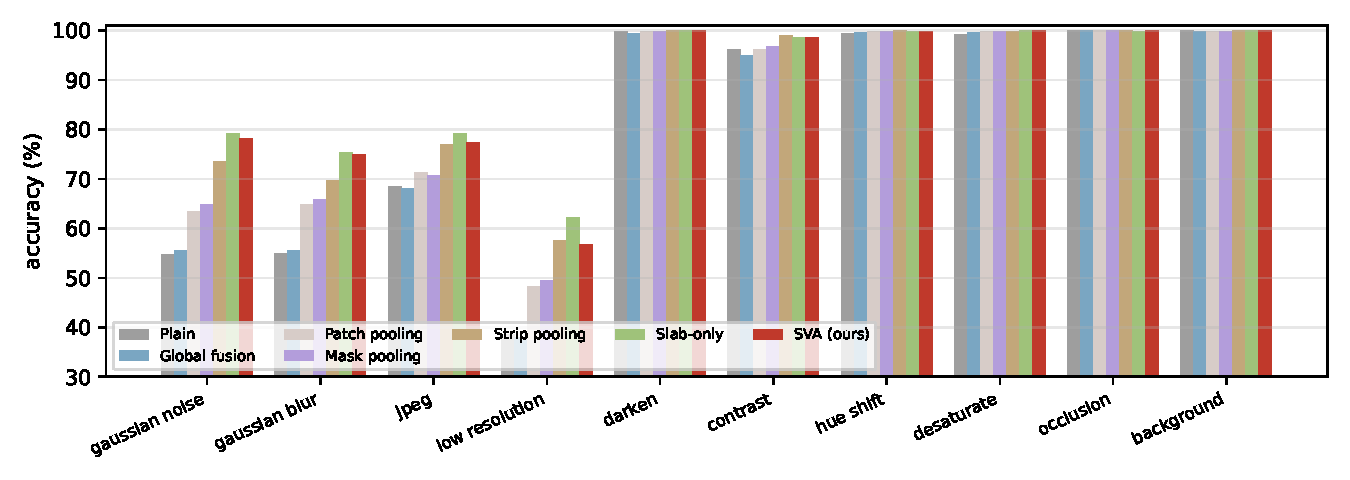
\includegraphics[width=\linewidth]{figures/fig_corruptions.pdf}
\caption{MedLeaf-C accuracy per corruption family (ConvNeXt-T, severity-averaged).}
\label{fig:corruptions}
\end{figure}

\subsection{Inside \SVA{}: ablations}
\label{sec:abl}
\Cref{tab:abl} varies one ingredient of \SVA{} at a time (ConvNeXt-T). A single-seed screen on folds
0--2 (lower block) was followed by the four most informative ablations on all 5 folds $\times$ 3
seeds (upper block), compared with \SVA{} on the same runs. The screen overstated every effect,
because its \SVA{} reference happened to be strong (53.1\% raw vs.\ 49.3\% over all seeds). With
three seeds, a coarser sweep costs $5.1$ [$1.1$, $9.1$] raw points (15/15) and unit cell weights
$4.5$ [$-0.5$, $9.5$] (13/15); Euler tokens transfer slightly worse than area and perimeter ($-2.6$,
12/15, n.s.); and restricting attention to the slab is not needed (global attention 49.3\% vs.\
49.3\%). These effects concern the internal design of \SVA{}; as shown above, the full module is not
better than localised pooling without any measurement. The vein head reproduces its ridge-filter
supervision closely on held-out leaves (Pearson $r=0.96$, Dice $0.74$--$0.75$ inside the blade),
which measures agreement with the pseudo-label, not with traced veins.

\begin{table}[t]
\centering
\caption{Ablations of \SVA{} (ConvNeXt-T, \%), each block sorted by raw field accuracy and compared
with \SVA{} on the same runs. Rotation is evaluated on seed 0 only.}
\label{tab:abl}
\small
\resizebox{\linewidth}{!}{\begin{tabular}{lcccc}
\toprule
Variant & Clean & Rot.\ min & Field (mask) & Field (raw) \\
\midrule
SVA (full) & 99.9\,$\pm$\,0.2 & 99.9\,$\pm$\,0.2 & 47.0\,$\pm$\,0.7 & 53.1\,$\pm$\,2.7 \\
softer relaxation ($\kappa{=}1$) & 100.0\,$\pm$\,0.0 & 99.9\,$\pm$\,0.2 & 46.8\,$\pm$\,1.1 & 52.5\,$\pm$\,2.1 \\
attention over all leaf patches & 100.0\,$\pm$\,0.0 & 100.0\,$\pm$\,0.0 & 47.1\,$\pm$\,1.1 & 52.0\,$\pm$\,2.5 \\
weights permuted within the leaf & 100.0\,$\pm$\,0.0 & 100.0\,$\pm$\,0.0 & 44.5\,$\pm$\,0.8 & 50.8\,$\pm$\,1.1 \\
venation field only & 99.9\,$\pm$\,0.2 & 99.8\,$\pm$\,0.2 & 45.3\,$\pm$\,0.6 & 50.7\,$\pm$\,2.5 \\
sharper relaxation ($\kappa{=}16$) & 100.0\,$\pm$\,0.0 & 99.9\,$\pm$\,0.2 & 46.5\,$\pm$\,2.6 & 50.6\,$\pm$\,3.8 \\
blade only & 100.0\,$\pm$\,0.0 & 99.9\,$\pm$\,0.2 & 43.8\,$\pm$\,2.0 & 48.4\,$\pm$\,4.1 \\
coarse sweep ($K{=}16,T{=}8$) & 100.0\,$\pm$\,0.0 & 99.9\,$\pm$\,0.2 & 43.2\,$\pm$\,1.2 & 46.8\,$\pm$\,1.0 \\
Euler token & 100.0\,$\pm$\,0.0 & 100.0\,$\pm$\,0.0 & 43.0\,$\pm$\,0.7 & 45.7\,$\pm$\,2.8 \\
Hadwiger token (area, perimeter, Euler) & 100.0\,$\pm$\,0.0 & 100.0\,$\pm$\,0.0 & 38.9\,$\pm$\,1.1 & 44.3\,$\pm$\,1.5 \\
unit cell weights & 99.9\,$\pm$\,0.2 & 99.8\,$\pm$\,0.2 & 41.5\,$\pm$\,1.2 & 43.5\,$\pm$\,0.7 \\
\bottomrule
\end{tabular}}
\end{table}

\subsection{Topology sensitivity}
\label{sec:topo}
The topology-destruction probe compares edits that change the blade's Euler characteristic (three
interior holes, $\Delta\chi=-3$) with edits that remove the same area from the margin ($\Delta\chi=0$).
The two edit types are not perceptually identical (median LPIPS 0.045 vs.\ 0.030), so we compare them
only within LPIPS strata that contain both (10 quantile bins, at least five edits of each kind) and
report the stratum-weighted log-ratio of the prediction change (KL divergence),
$\log(\mathrm{KL}_{\text{holes}}/\mathrm{KL}_{\text{bites}})$, with a bootstrap 95\% interval
(\cref{tab:topo}). Every ImageNet ConvNeXt-T and ViT-S model responds \emph{less} to holes than to
margin bites, even though the holes are the more visible edit. The only ConvNeXt-T model that responds
more to holes is the Euler-token variant of \SVA{} ($+0.73$ [$+0.54$, $+0.96$]), so measured topology
does change what a model is sensitive to. BioCLIP~2 responds more to holes for every variant ($+1.3$ to
$+1.6$), i.e.\ the foundation model is topology-sensitive by itself. Topological sensitivity can thus
be induced, but it did not help species transfer (\cref{sec:abl}). Edits of the venation could not be
matched perceptually (only 25\% of vein edits fall inside the LPIPS range of their controls), so we
draw no conclusion from them.

\begin{table}[t]
\centering
\caption{LPIPS-matched response to topology-changing holes relative to area-matched margin bites,
$\log(\mathrm{KL}_{\text{holes}}/\mathrm{KL}_{\text{bites}})$ with bootstrap 95\% CI (seed 0, 5 folds).
Negative: the model reacts more to margin geometry than to topology.}
\label{tab:topo}
\small
\begin{tabular}{llc}
\toprule
Backbone & Model & log-ratio [95\% CI] \\
\midrule
ConvNeXt-T & Plain & -1.22 [-1.47, -1.02] \\
 & Global fusion & -0.95 [-1.15, -0.75] \\
 & Strip pooling & -0.90 [-1.02, -0.77] \\
 & Slab-only & -0.96 [-1.11, -0.81] \\
 & SVA & -1.63 [-1.76, -1.48] \\
 & Euler token (ablation) & +0.73 [+0.54, +0.96] \\
\midrule
ViT-S/16 & Plain & -0.35 [-0.51, -0.22] \\
 & Global fusion & -0.62 [-0.76, -0.49] \\
 & Strip pooling & -0.84 [-1.03, -0.65] \\
 & Slab-only & -0.70 [-0.88, -0.52] \\
 & SVA & -0.42 [-0.60, -0.25] \\
\midrule
BioCLIP 2 & Plain & +1.63 [+1.50, +1.76] \\
 & Global fusion & +1.47 [+1.34, +1.60] \\
 & Strip pooling & +1.34 [+1.23, +1.45] \\
 & Slab-only & +1.36 [+1.23, +1.50] \\
 & SVA & +1.60 [+1.46, +1.74] \\
\bottomrule
\end{tabular}
\end{table}

\subsection{Leakage audit}
\label{sec:leak}
Under random image-level splits that keep the duplicates, 5--11 test images per fold (1.4--3.0\%) have
an exact duplicate or a re-shot of the same leaf in the training part; under our grouped protocol
there are none. On this dataset the leak does not measurably inflate accuracy: a DeepHerb-style
reproduction (Xception features with an RBF-SVM~\citep{roopashree2021deepherb}) reaches
$98.5\pm0.9\%$ with random splits and $98.4\pm0.7\%$ with grouped splits, the dual-branch RGB +
vein-skeleton baseline~\citep{dualbranch2026} reaches 99.95\% under both, and our plain and \SVA{}
models reach 100\% under random splits as under grouped ones. We therefore present the grouped protocol
as hygiene that removes a known leak rather than as evidence that earlier results were inflated; the
saturation itself is the more important observation.
